\chapter{A new mesh for representing the atmosphere above terrain}
\label{ch:slanted}

\begin{highlights}
{\Large Highlights}
\begin{itemize}
	\item The new slanted cell mesh permits longer time-steps than cut cells, with time-steps comparable to terrain-following meshes
	\item \TODO{Pressure gradient calculations are more accurate using slanted cells compared to BTF meshes --- but not SLEVE! this is a weak conclusion!}
	\item Unlike the multidimensional linear upwind scheme, the cubicFit scheme is numerically stable over very steep slopes
\end{itemize}
\end{highlights}

\TODO{
Motivation
\begin{itemize}
	\item cut cells can improve pressure gradient accuracy over TF layers, but they have arbitrarily small cells and they're not simple to construct
	\item we seek a mesh that improves pressure gradient errors, but avoids arbitrarily small cells and is easier to construct than cut cell meshes
	\item to ensure cubicFit is numerically stable and accurate on slanted cell meshes with steep slopes, we transport a tracer along the ground through the slanted cells
\end{itemize}
}

\TODO{The new resting atmosphere results with steeper mountains make slantedCells unattractive compared to SLEVE or cut cells.  So now there are no tests in which slanted cells outperform other meshes.  I see three options here:
\begin{enumerate}
\item Keep the weak conclusion that slanted cells aren't very good.
\item Formulate and implement a better cell merging method to better control pressure gradient errors.
\item Present two sets of slanted cell results in the resting atmosphere test: one with tolerance=0 and another with tolerance=2dx/5.  I already know that results are more stable and accurate when tolerance=2dz/5 is used to remove the thinnest slanted cells.  This crude thin-cell-avoidance method is quite effective, therefore we'd expect a better cell merging method to help further still.
\end{enumerate}
}

\vspace*{-1em}
\section{Transport over a mountainous lower boundary}
\label{sec:slanted:mountainAdvect}

The two-dimensional tests performed in chapter~\ref{ch:cubicFit} transported tracers positioned well above the terrain surface.  Here we formulate a new test, positioning the tracer at the ground in order to assess the accuracy of transport schemes immediately above a mountainous lower boundary.  Results are compared between the cubicFit scheme and the linearUpwind scheme on basic terrain-following, cut cell and slanted cell meshes.
The test presents a particular challenge to transport schemes as they must transport the tracer through arbitrarily small cut cells and distorted slanted cells.

The domain size and mountain profile are the same as those in the horizontal tracer transport test in section~\ref{sec:cubicFit:schaerAdvect}, with a mesh spacing of $\Delta x = \SI{1000}{\meter}$ and $\Delta z = \SI{500}{\meter}$.
In order to present the most challenging test on slanted cell meshes vertices are not moved downwards, and so thin cells remain near mountain peaks.
Cell edges in the central region of the domain are shown in figure~\ref{fig:slanted:mountainAdvect:meshes} for each of the three mesh types.
Cells in the BTF mesh are highly distorted over steep slopes (figure~\ref{fig:slanted:mountainAdvect:meshes:btf}) while the cut cell mesh (figure~\ref{fig:slanted:mountainAdvect:meshes:cutCell}) and slanted cell mesh (figure~\ref{fig:slanted:mountainAdvect:meshes:slantedCell}) are orthogonal everywhere except for cells nearest the ground.

\begin{figure}
	\centering
	\begin{subfigure}{\textwidth}
		\phantomsubcaption\label{fig:slanted:mountainAdvect:meshes:btf}
		\phantomsubcaption\label{fig:slanted:mountainAdvect:meshes:cutCell}
		\phantomsubcaption\label{fig:slanted:mountainAdvect:meshes:slantedCell}
		\centering
		\includegraphics{thesis/slanted/mountainAdvect/fig-meshes.pdf}
	\end{subfigure}
%
	\caption{Two dimensional $x$-$z$ meshes created with the (\subcaptionref{fig:slanted:mountainAdvect:meshes:btf}) basic terrain-following,
	(\subcaptionref{fig:slanted:mountainAdvect:meshes:cutCell}) cut cell, and
	(\subcaptionref{fig:slanted:mountainAdvect:meshes:slantedCell}) slanted cell methods, used for the tracer transport tests in section~\ref{sec:slanted:mountainAdvect}.  Cell edges are marked by thin black lines.  The peak mountain height $h_0 = \SI{5}{\kilo\meter}$.
The velocity field is the same for all mesh types with streamlines marked on each panel by thick red lines.
The velocity field (equation~\ref{eqn:streamfunc-btf}) follows the lower boundary and becomes entirely horizontal above $H_1 = \SI{10}{\kilo\meter}$.
	\rev{The mesh spacing is $\Delta x = \SI{1000}{\meter}$ and $\Delta z = \SI{500}{\meter}$.}
Only the lowest \SI{10}{\kilo\meter} for the central region of the domain is shown.  The entire domain is \SI{300}{\kilo\meter} wide and \SI{25}{\kilo\meter} high.}
	\label{fig:slanted:mountainAdvect:meshes}
\end{figure}

A velocity field is prescribed using equation~\eqref{eqn:streamfunc-btf} so that the flow follows the terrain at the surface and becomes entirely horizontal above $H_1 = \SI{10}{\kilo\meter}$.
The value of $H_1$ is chosen to be much smaller than the domain height $H$ in equation~\eqref{eqn:btf} so that flow crosses the surfaces of the BTF mesh.
This is evident in figure~\ref{fig:slanted:mountainAdvect:meshes:btf} where the the velocity streamlines are tangential to the mesh only at the ground.
The flow is deliberately misaligned with the BTF, cut cell and slanted cell meshes away from the ground (figure~\ref{fig:slanted:mountainAdvect:meshes}) to ensure that flow always crosses mesh surfaces in order to challenge the transport schemes.

\begin{table}
	\centering
	\input{slanted/mountainAdvect/timesteps}
%
	\caption{Time-steps (\si{\second}) for the two-dimensional transport test over a mountainous lower boundary.  The time-steps were chosen so that the maximum Courant number was between \num{0.36} and \num{0.46}.}
	\label{tab:slanted:mountainAdvect:timesteps}
\end{table}

The tracer is defined again by equation~\eqref{eqn:cubicFit:schaerAdvect:tracer} but is now positioned at the ground with $(x_0, z_0) = (\SI{-50}{\kilo\meter}, \SI{0}{\kilo\meter})$ with half-widths $A_x = \SI{25}{\kilo\meter}$ and $A_z = \SI{10}{\kilo\meter}$.
Tests are integrated forward for \SI{10000}{\second}.  The time-step was chosen for each mesh so that the maximum Courant number was about \num{0.4} (table~\ref{tab:slanted:mountainAdvect:timesteps}).
An analytic solution at \SI{10000}{\second} is obtained by calculating the new horizontal position of the tracer using equation~\eqref{eqn:cubicFit:tfAdvect:trajectory}.
By solving this equation we find that \(x(t=\SI{10000}{\second}) = \SI{6244.087}{\meter}\) when $h_0 = \SI{5}{\kilo\meter}$.

The tracer density boundary conditions are the same as those in section~\ref{sec:cubicFit:schaerAdvect}.
Since the cubicFit transport scheme uses values at boundaries with Dirichlet boundary conditions, the cubicFit scheme uses only inlet boundary values in this test case.

\begin{figure}
	\centering
	\includegraphics{thesis/slanted/mountainAdvect/fig-tracer.pdf}
	%
	\caption{Evolution of the tracer in the two-dimensional transport test over a mountainous lower boundary.  The tracer is transported to the right over the wave-shaped terrain.  Tracer contours are every \SI{0.1}{\kilo\gram\per\meter\cubed}.  The result obtained using the cubicFit scheme on the basic terrain-following mesh is shown at $t=\SI{0}{\second}$, $t=\SI{5000}{\second}$ and $t=\SI{10000}{\second}$ with solid black contours. The analytic solution at $t=\SI{10000}{\second}$ is shown with dotted contours.
	\rev{The mesh spacing is $\Delta x = \SI{1000}{\meter}$ and $\Delta z = \SI{500}{\meter}$.}
	The shaded box indicates the region that is plotted in figure~\ref{fig:slanted:mountainAdvect:errors}.}
	\label{fig:slanted:mountainAdvect:tracer}
\end{figure}

Three series of tests were performed using similar configurations.  The first series uses a peak mountain height of $h_0 = \SI{5}{\kilo\meter}$ to examine errors on different mesh types using the linearUpwind and cubicFit transport schemes.
The second series varies the peak mountain height to examine the sensitivity of the two transport schemes to mesh distortions.
The third series verifies accuracy at Courant numbers close to the limit of stability, and examines the longest stable time-step for different mesh types.

\subsection{Comparison of numerical accuracy between mesh types and transport schemes}
For the first series of tests with $h_0 = \SI{5}{\kilo\meter}$, tracer contours at the initial time $t=\SI{0}{\second}$, half-way time $t=\SI{5000}{\second}$, and end time $t=\SI{10000}{\second}$ are shown in figure~\ref{fig:slanted:mountainAdvect:tracer} using the cubicFit scheme on the BTF mesh.  As apparent at $t=\SI{5000}{\second}$, the tracer is distorted by the terrain-following velocity field as it passes over the mountain as expected, and its original shape is restored once it has cleared the mountain by $t=\SI{10000}{\second}$.
Slight errors are apparent at $t = \SI{10000}{\second}$ when the numerical solution marked with solid contour lines is compared with the analytic solution marked with dotted contour lines.

\begin{figure}
	\begin{subfigure}{\textwidth}
		\centering
		\phantomsubcaption\label{fig:slanted:mountainAdvect:errors:linearUpwind-btf}
		\phantomsubcaption\label{fig:slanted:mountainAdvect:errors:linearUpwind-cutCell}
		\phantomsubcaption\label{fig:slanted:mountainAdvect:errors:linearUpwind-slantedCell}
		\phantomsubcaption\label{fig:slanted:mountainAdvect:errors:cubicFit-btf}
		\phantomsubcaption\label{fig:slanted:mountainAdvect:errors:cubicFit-cutCell}
		\phantomsubcaption\label{fig:slanted:mountainAdvect:errors:cubicFit-slantedCell}
		%
		\includegraphics{thesis/slanted/mountainAdvect/fig-error.pdf}
	\end{subfigure}

	\caption{Tracer contours at $t=\SI{10000}{\second}$ for the two-dimensional tracer transport tests over a mountainous lower boundary.  A region in the lee of the mountain is plotted corresponding to the shaded area in figure~\ref{fig:slanted:mountainAdvect:tracer}.
	Results are presented on BTF, cut cell and slanted cell meshes (shown in figure~\ref{fig:slanted:mountainAdvect:meshes}) using the linearUpwind and cubicFit transport schemes.  The numerical solutions are marked by solid black lines.  The analytic solution is marked by dotted lines.  Contours are every \SI{0.1}{\kilo\gram\per\meter\cubed}.
	\rev{The mesh spacing is $\Delta x = \SI{1000}{\meter}$ and $\Delta z = \SI{500}{\meter}$.}
	}
	\label{fig:slanted:mountainAdvect:errors}
\end{figure}

Numerical errors are more clearly revealed by subtracting the analytic solution from the numerical solution.
Error fields are compared between BTF, cut cell and slanted cell meshes using the linearUpwind scheme (figures~\ref{fig:slanted:mountainAdvect:errors:linearUpwind-btf},
\ref{fig:slanted:mountainAdvect:errors:linearUpwind-cutCell} and
\ref{fig:slanted:mountainAdvect:errors:linearUpwind-slantedCell} respectively) and the cubicFit scheme (figures~\ref{fig:slanted:mountainAdvect:errors:cubicFit-btf},
\ref{fig:slanted:mountainAdvect:errors:cubicFit-cutCell} and
\ref{fig:slanted:mountainAdvect:errors:cubicFit-slantedCell} respectively).
Results are least accurate using the linearUpwind scheme on the slanted cell mesh (figure~\ref{fig:slanted:mountainAdvect:errors:linearUpwind-slantedCell}) with the final tracer being slightly distorted.
The $\ell_\infty$ error magnitude is reduced by using the linearUpwind scheme on the cut cell mesh (figure~\ref{fig:slanted:mountainAdvect:errors:linearUpwind-cutCell}), but the shape of the error remains the same.
On the BTF mesh (figure~\ref{fig:slanted:mountainAdvect:errors:cubicFit-btf}), cut cell mesh (figure~\ref{fig:slanted:mountainAdvect:errors:cubicFit-cutCell}) and slanted cell mesh (figure~\ref{fig:slanted:mountainAdvect:errors:cubicFit-slantedCell}), the cubicFit scheme is more accurate than the linearUpwind scheme.

\subsection{Numerical stability and numerical accuracy with increasingly steep slopes}

\begin{figure}
	\centering
	\input{slanted/mountainAdvect/l2ByMountainHeight}
%
	\caption{Error measures for the two-dimensional tracer transport tests over a mountainous lower boundary.  Peak mountain heights $h_0$ are from \SIrange{0}{6}{\kilo\meter}.  Results are compared on BTF, cut cell and slanted cell meshes using the linearUpwind and the cubicFit schemes.  At $h_0 = \SI{0}{\kilo\meter}$ the terrain is entirely flat and the BTF, cut cell and slanted cell meshes are identical.  At $h_0 = \SI{6}{\kilo\meter}$ the linearUpwind scheme is unstable on the slanted cell mesh.}
	\label{fig:slanted:mountainAdvect:l2ByMountainHeight}
\end{figure}

To further examine the performance of the cubicFit scheme in the presence of steep terrain, a second series of tests were performed in which the peak mountain height was varied from \SIrange{0}{6}{\kilo\meter} keeping all other parameters constant.
Results were obtained on BTF, cut cell and slanted cell meshes using the linearUpwind scheme and cubicFit scheme.  Again, the time-step was chosen for each test so that the maximum Courant number was about \num{0.4} (table~\ref{tab:slanted:mountainAdvect:timesteps}).  The $\ell_2$ error was calculated by subtracting the analytic solution from the numerical solution (figure~\ref{fig:slanted:mountainAdvect:l2ByMountainHeight}).
Note that the analytic solution is a function of mountain height, with the tracer travelling farther over higher mountains due to non-divergent flow through a narrower channel.
In all cases, error increases with increasing mountain height because steeper slopes lead to greater mesh distortions.
Errors are identical for a given transport scheme when $h_0 = \SI{0}{\kilo\meter}$ and the ground is entirely flat because the BTF, cut cell and slanted cell meshes are identical.
The linearUpwind scheme is unstable on the slanted cell mesh with a peak mountain height $h_0 = \SI{6}{\kilo\meter}$ despite using a Courant number of \inputval{mountainAdvect-h0-slantedCell-1000-6000m-linearUpwind/co}\unskip.
The cubicFit scheme yields stable results in all tests, and cubicFit is more accurate than linearUpwind in all tests.

\subsection{Numerical stability limits of the cubicFit transport scheme}

\begin{figure}
	\begin{subfigure}{\textwidth}
		\centering
		\input{slanted/mountainAdvect/maxdt}
		\phantomsubcaption\label{fig:slanted:mountainAdvect:maxdt:dt}
		\phantomsubcaption\label{fig:slanted:mountainAdvect:maxdt:co}
	\end{subfigure}
	%
	\caption{(\subcaptionref{fig:slanted:mountainAdvect:maxdt:dt}) Longest stable time-steps, $\Delta t_\mathrm{max}$, and 
	(\subcaptionref{fig:slanted:mountainAdvect:maxdt:co}) largest stable maximum Courant numbers, $\max(\mathrm{Co})$, for the two-dimensional tracer transport test over a mountainous lower boundary.  Results were obtained on basic terrain-following, cut cell and slanted cell meshes at mesh spacings between $\Delta x = \SI{5000}{\meter}$ and $\Delta x = \SI{250}{\meter}$.  The largest stable maximum Courant numbers were calculated from the corresponding longest stable time-steps using equation~\eqref{eqn:co}.
	\rev{The peak mountain height $h_0 = \SI{6}{\kilo\meter}$.}}
	\label{fig:slanted:mountainAdvect:maxdt}
\end{figure}

A final series of tests were performed to determine the stability limit of the cubicFit scheme with the two-stage Heun time-stepping scheme (equation~\ref{eqn:heun}).
The tracer was transported on BTF, slanted cell and cut cell meshes with a variety of mesh spacings between $\Delta x = \SI{5000}{\meter}$ and $\Delta x = \SI{125}{\meter}$.  $\Delta z$ was chosen so that a constant aspect ratio is preserved such that $\Delta x \mathbin{:} \Delta z = 2 \mathbin{:} 1$.
\rev{The peak mountain height $h_0 = \SI{6}{\kilo\meter}$.}
For each test, the time-step was adjusted in order to find the largest stable time-step, $\Delta t_\mathrm{max}$ (figure~\ref{fig:slanted:mountainAdvect:maxdt:dt}).
BTF meshes permit the longest time-steps of all three mesh types since cells are almost uniform in volume.  As expected, the longest stable time-step scales linearly with BTF mesh spacing.
There is no such linear scaling on cut cell meshes because these meshes can have arbitrarily small cells.  The time-step constraints on cut cell meshes are the most severe of the three mesh types.  Slanted cell meshes have a slightly more stringent time-step constraint than BTF meshes but still exhibit similar linear scaling with mesh spacing.

Figure~\ref{fig:slanted:mountainAdvect:maxdt:co} presents the largest stable maximum Courant numbers, $\max(\mathrm{Co})$, which were calculated by substituting $\Delta t = \Delta t_\mathrm{max}$ into equation~\eqref{eqn:co}.
On basic terrain-following meshes, the maximum Courant number tends towards about \num{1.3} with finer mesh spacings.
No such trend is found on cut cell or slanted cell meshes.
Cut cell meshes permit the largest maximum Courant numbers of around \num{3}, but the largest stable time-steps on cut cell meshes are still smaller than corresponding time-steps on basic terrain-following and slanted cell meshes.

This thesis focuses on the spatial discretisation of the cubicFit scheme, but the stability limit depends also upon the choice of time-stepping.  We have not calculated a theoretical Courant number limit, although such an analysis should be possible using the techniques of \citet{baldauf2008}.

This new test case demonstrates that the cubicFit transport scheme is more accurate than the linearUpwind scheme on all meshes, and only the cubicFit scheme can achieve stable results on slanted cell meshes with very steep slopes.
The slanted cell method exhibits a time-step constraint that scales linearly with mesh spacing, and slanted cells avoid severe time-step constraints associated with arbitrarily small cut cells.
Next, we incorporate the cubicFit transport scheme into a model of the fully compressible Euler equations.

\section{Stratified atmosphere initially at rest}
\label{sec:slanted:resting}

Diurnal valley and slope flows are associated with weak synoptic-scale winds, and cold air that sinks along sloping terrain can stagnate for days after becoming trapped in topographic basins \citep{chow2013}.
The test case by \citet{klemp2011} is an idealised representation of such phenomena, in which a wave-shaped mountain is submerged in a stably stratified atmosphere at rest in hydrostatic balance.
The analytic solution is time-invariant, but numerical errors in calculating pressure gradients can give rise to spurious flows which become stronger over steeper terrain \citep{klemp2011}.
Results are compared using terrain-following, cut cell and slanted cell meshes.

Following \cite{klemp2011}, the domain is \SI{200}{\kilo\meter} wide and \SI{20}{\kilo\meter} high, and the mesh spacing is \(\Delta x = \Delta z^\star = \SI{500}{\meter}\).  All boundary conditions are no normal flow.
The wave-shaped mountain profile has a surface height, $h$, given by
\begin{align}
	h(x) = h_0 \exp \left( - \left( \frac{x}{a} \right)^2 \right) \cos^2 \left( \alpha x \right) \label{eqn:resting:mountain}
\end{align}
where $a = \SI{5}{\kilo\meter}$ is the mountain half-width $\lambda = \SI{4}{\kilo\meter}$ is the wavelength and $h_0$ is the peak mountain height.  For the optimised SLEVE mesh, the coarse-scale component $h_1$ is specified as
\begin{align}
	h_1(x) = \frac{1}{2} h_0 \exp \left( - \left( \frac{x}{a} \right)^2 \right) \text{ .}
\end{align}
To accommodate a range of mountain heights we choose a coarse scale height $s_1 = \SI{20}{\kilo\meter}$ and a fine scale height $s_2 = \SI{8}{\kilo\meter}$.  Following \citet{leuenberger2010} the optimal exponent value of $n = \num{1.35}$ is used.  These parameter values result in a SLEVE mesh that is more distorted than the SLEVE mesh used by \citet{klemp2011}, but the choice is necessary to avoid mesh tangling with mountains higher than \SI{1}{\kilo\meter}.

The initial potential temperature field has a nonlinear vertical profile in the lower atmosphere, with $\theta(z = 0) = \SI{288}{\kelvin}$ and a constant static stability with Brunt-V\"ais\"al\"a frequency $N = \SI{0.01}{\per\second}$ everywhere, except for a more stable layer of $N = \SI{0.02}{\per\second}$ between $\SI{2}{\kilo\meter} \leq z \leq \SI{3}{\kilo\meter}$.
The Exner function of pressure is calculated so that it is in discrete hydrostatic balance in the vertical direction \citep{weller-shahrokhi2014}.  The damping function \(\mu\) is set to \SI{0}{\per\second}.  Unlike \citet{klemp2011}, there is no eddy diffusion in the equation set.

\begin{figure}
	\centering
	\begin{subfigure}{\textwidth}
		\centering
		\input{slanted/resting/w}
		\phantomsubcaption\label{fig:slanted:resting:w:timeseries}
		\phantomsubcaption\label{fig:slanted:resting:w:max}
	\end{subfigure}
	\caption{Spurious vertical velocities in the resting atmosphere test using BTF, SLEVE, cut cell and slanted cell meshes.
	(\subcaptionref{fig:slanted:resting:w:timeseries}) Time series of spurious vertical velocities for a peak mountain height $h_0 = \SI{1}{\kilo\meter}$, with the maximum absolute value calculated at each time-step. 
	(\subcaptionref{fig:slanted:resting:w:max}) Sensitivity to peak mountain height $h_0$, with the maximum absolute value calculated across all time-steps.
	}
	\label{fig:slanted:resting:w}
\end{figure}

The test is integrated forward by \num{6} hours using a time-step of $\Delta t = \SI{25}{\second}$ on the BTF, SLEVE, cut cell and slanted cell meshes with a peak mountain height $h_0 = \SI{1}{\kilo\meter}$.
For each mesh, the maximum absolute vertical velocity is calculated at each time-step as a measure of the spurious flow generated by numerical errors.  In agreement with \citep{klemp2011}, magnitudes of vertical velocity peak shortly after integration begins and magnitudes are larger on more distorted meshes (figure~\ref{fig:slanted:resting:w:timeseries}).
However, magnitudes are much smaller comparing results on the terrain-following meshes with those from \citet{klemp2011}: results in figure~\ref{fig:slanted:resting:w:timeseries}, which use a curl-free pressure gradient formulation, have maximum absolute vertical velocities of \inputval{resting-btf-1000m-cubicFit/maxw}\unskip, compared with a maximum of $\sim \SI{7}{\meter\per\second}$ found by \citet{klemp2011} using their improved horizontal pressure gradient formulation.
The results on terrain-following meshes in figure~\ref{fig:slanted:resting:w:timeseries} have similar maximum errors as \citet{weller-shahrokhi2014} but, due to the more stable split into implicitly and explicitly treated terms (described in the appendix to \citet{shaw-weller2016}), the errors decay over time due to the dissipative nature of the transport scheme.
Unlike the result from \citet{klemp2011}, spurious flows are similar on both terrain-following meshes even though the SLEVE mesh is less distorted than the BTF mesh.

Compared to results on the terrain-following meshes, spurious flows are two orders of magnitude smaller on the cut cell mesh and the slanted cell mesh with a maximum absolute vertical velocity of $\sim \SI{1e-3}{\meter\per\second}$.
\citet{good2014} found the maximum vertical velocity in their cut cell model was \SI{1e-12}{\meter\per\second}, which is better than any result obtained here.  It is worth noting that our model stores values at the geometric centre of cut cells, whereas the model used by \citet{good2014} has cell centres at the centre of the uncut cell, resulting in the centre of some cut cells being below the ground (S.-J. Lock 2014, personal communication).
This means that the mesh is effectively regular when calculating horizontal and vertical gradients, and this would account for the very small velocities found by \citet{good2014}.

To evaluate the slanted cell method with steeper slopes, we perform a second series of tests with peak mountain heights ranging from $h_0 = \SI{0}{\kilo\meter}$ to $h_0 = \SI{6}{\kilo\meter}$.
The BTF, SLEVE, cut cell and slanted cell meshes with the largest peak mountain height of $h_0 = \SI{6}{\kilo\meter}$ are shown in figure~\ref{fig:slanted:resting:meshes}.
To obtain a single measure of spurious flow for a given mesh, the maximum absolute vertical velocity is calculated across all time-steps.
The most accurate results are obtained without mountains when $h_0 = \SI{0}{\kilo\meter}$ when all meshes become identical, with $\max(\Mag{w}) \sim \SI{1e-11}{\meter\per\second}$.
Using terrain-following meshes, the model becomes unstable beyond $h_0 = \SI{2}{\kilo\meter}$.
Using cut cell meshes, maximum vertical velocities are almost constant at $\sim \SI{0.5}{\meter\per\second}$ beyond $h_0 = \SI{1}{\kilo\meter}$ because cut cell mesh distortions are largely independent of mountain height.
Using slanted cell meshes, maximum vertical velocities are one to two orders of magnitude smaller than those found on terrain-following meshes at a given mountain height.  Unlike results on terrain-following meshes, slanted cell meshes yield stable results for all mountain heights, although maximum vertical velocities increase with peak mountain height as slanted cells become increasingly distorted.  Up to a peak mountain height of $h_0 = \SI{4}{\kilo\meter}$, slanted cell meshes produce results that are more accurate than those obtained for any other mesh.

In summary, spurious velocities in the resting atmosphere test were similar on both terrain-following meshes, with errors being much smaller compared to those from \citet{klemp2011}.
The maximum absolute vertical velocity was decreased by one to two orders of magnitude using cut cell and slanted cell meshes, so we conclude that, in this test, mesh distortion, or lack of alignment of the mesh with surfaces of constant gravitational potential, are the primary cause of numerical error.
The resting atmosphere test presented a challenge to the pressure gradient formulation but the resultant spurious flows presented no particular challenge to the cubicFit transport scheme.  We will turn our attention to transport-dominated flow in the next chapter.

\section{Sch\"{a}r mountain waves test}
\label{sec:cp:schaerWaves}

Chapter~\ref{ch:slanted} assessed a finite volume model of the fully compressible Euler equations with a Lorenz staggering using a test case with a stratified atmosphere initially at rest above an isolated mountain.
We now turn our attention to a transport-dominated test case that presents a challenge to the transport schemes within the dynamical model.
As specified by \citet{schaer2002}, the test prescribes flow over idealised terrain with small-scale and large-scale undulations that induce propagating and evanescent gravity waves.
We use the test to compare results from the two finite volume model variants with Lorenz and generalised Charney--Phillips staggerings against the reference solution from \citet{melvin2010}.

Following \citet{melvin2010}, the domain is \SI{300}{\kilo\meter} wide and \SI{30}{\kilo\meter} high, and the mesh spacing is $\Delta x = \SI{500}{\meter}$ and $\Delta z^\star = \SI{300}{\meter}$.
The mountain profile has the same form as equation~\eqref{eqn:resting:mountain}, but the mountain waves test has a lower peak mountain height of $h_0 = \SI{250}{\meter}$.  As in the resting atmosphere test (section~\ref{sec:slanted:resting}), $a = \SI{5}{\kilo\meter}$ is the mountain half-width and $\lambda = \SI{4}{\kilo\meter}$ is the wavelength.

A uniform horizontal wind $(u, w) = (10, 0)\:\si{\meter\per\second}$ is prescribed in the domain interior and at the inlet boundary.  No normal flow is imposed at the top and bottom boundaries and the velocity field has a zero gradient outlet boundary condition.

The initial thermodynamic conditions have constant static stability with $N = \SI{0.01}{\per\second}$ everywhere such that
\begin{align}
	\theta(z) = \theta_0 \exp \left( \frac{N^2}{g} z \right) \label{eqn:cp:schaerWaves:thermal-profile}
\end{align}
where the temperature at $z=0$ is $\theta_0 = \SI{288}{\kelvin}$.
Potential temperature values are prescribed at the inlet and upper boundary using equation~\eqref{eqn:cp:schaerWaves:thermal-profile}, and a zero gradient boundary condition is applied at the outlet.
At the ground, fixed gradients are imposed by calculating the component of $\nabla \theta$ normal to each face using the vertical derivative of equation~\eqref{eqn:cp:schaerWaves:thermal-profile}.
For the Exner function of pressure, hydrostatic balance is prescribed on top and bottom boundaries and the inlet and outlet are zero normal gradient.

Sponge layers are added to the upper \SI{10}{\kilo\meter} and leftmost \SI{10}{\kilo\meter} at the inlet boundary to damp the reflection of waves.
The damping term \(\mu\) in the momentum equation \eqref{eqn:exnerFoam:momentum} is a function adapted from \citet{melvin2010} such that
\begin{subequations}
\begin{align}
	\mu(x, z) &= \mu_\mathrm{upper} + \mu_\mathrm{inlet} \\
	\mu_\mathrm{upper}(z) &= \begin{cases}
		\overline{\mu} \sin^2 \left( \frac{\pi}{2} \frac{z - z_B}{H - z_B} \right) & \enskip \text{if $z \geq z_B$,} \\
		0 & \enskip \text{otherwise,} \\
	\end{cases} \\
	\mu_\mathrm{inlet}(x) &= \begin{cases}
		\overline{\mu} \sin^2 \left( \frac{\pi}{2} \frac{x_I - x}{x_I - x_0} \right) & \enskip \text{if $x < x_I$,} \\
		0 & \enskip \text{otherwise,}
	\end{cases}
\end{align}%
\end{subequations}
where $\overline{\mu} = \SI{1.2}{\per\second}$ is the damping coefficient, $z_B = \SI{20}{\kilo\meter}$ is the bottom of the sponge layer, $H = \SI{30}{\kilo\meter}$ is the top of the domain, $x_0 = \SI{-150}{\kilo\meter}$ is the leftmost limit of the domain and $x_I = \SI{-140}{\kilo\meter}$ is the rightmost extent of the inlet sponge layer.
The sponge layer is active only on entirely horizontal faces so that only vertical momentum is damped.
Note that, while the domain itself is \SI{30}{\kilo\meter} in height, for the purposes of generating basic terrain-following meshes, the domain height is set to \SI{20}{\kilo\meter} because the sponge layer occupies the uppermost \SI{10}{\kilo\meter}.

\begin{figure}
	\centering
	\begin{subfigure}{0.55\textwidth}
		\centering
		\caption{Lorenz staggering, linearUpwind transport}
		\label{fig:cp:schaerWaves:w:linearUpwind}
		\includegraphics{thesis/cp/schaerWaves/fig-btf-300dz-linearUpwind-w.pdf}
	\end{subfigure}
	\begin{subfigure}{0.44\textwidth}
		\centering
		\caption{Lorenz staggering, cubicFit transport}
		\label{fig:cp:schaerWaves:w:cubicFit}
		\includegraphics{thesis/cp/schaerWaves/fig-btf-300dz-cubicFit-w.pdf}
	\end{subfigure}
	\\
	\vspace*{1em}
	%
	\begin{subfigure}{0.55\textwidth}
		\centering
		\caption{Generalised Charney--Phillips staggering}
		\label{fig:cp:schaerWaves:w:cp}
		\includegraphics{thesis/cp/schaerWaves/fig-btf-300dz-cp-w.pdf}
	\end{subfigure}
	\begin{subfigure}{0.44\textwidth}
		\centering
		\caption{Reference solution by \citet{melvin2010}}
		\label{fig:cp:schaerWaves:w:melvin}
		\raisebox{0.2in}{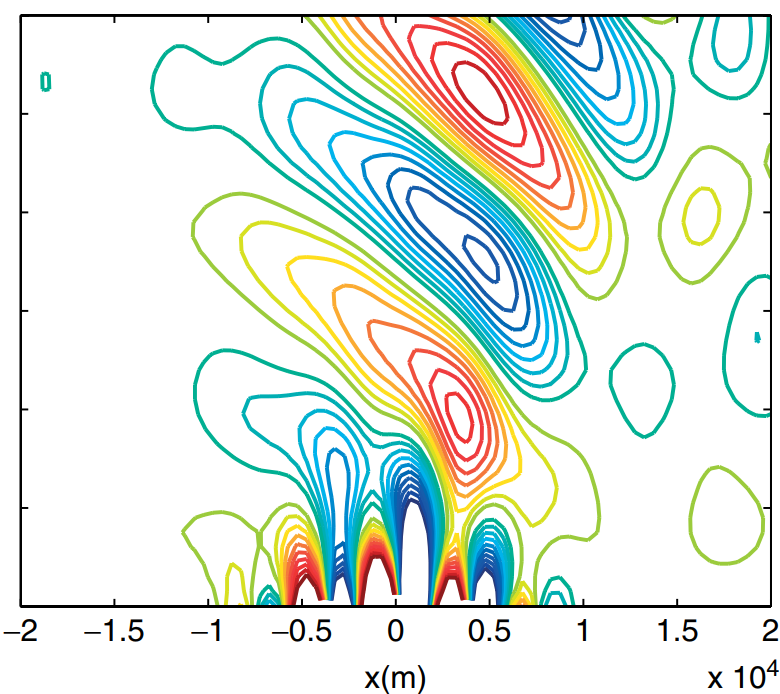
\includegraphics[height=1.9in]{cp/schaerWaves/melvin2010-w-mass-conserving-sisl.png}}
	\end{subfigure}
	\caption{Vertical velocities at the end of integration of the Sch\"{a}r mountain waves test case.
	Results obtained using a basic terrain-following mesh and Lorenz staggering, with potential temperature and momentum transported by (\subcaptionref{fig:cp:schaerWaves:w:linearUpwind}) the linearUpwind scheme and
	(\subcaptionref{fig:cp:schaerWaves:w:cubicFit}) the cubicFit scheme, and (\subcaptionref{fig:cp:schaerWaves:w:cp}) using a basic terrain-following mesh and generalised Charney--Phillips staggering.
	For comparison, (\subcaptionref{fig:cp:schaerWaves:w:melvin}) provides a reference solution obtained with a mass-conserving semi-implicit semi-Lagrangian model \citep{melvin2010}.
	Contours are plotted every \SI{0.05}{\meter\per\second}.  In figures (\subcaptionref{fig:cp:schaerWaves:w:linearUpwind}), (\subcaptionref{fig:cp:schaerWaves:w:cubicFit}) and (\subcaptionref{fig:cp:schaerWaves:w:cp}), ascending velocities are marked by solid black lines and descending velocities are marked by dashed red lines.
Only the lowest \SI{12}{\kilo\meter} in the central region of the domain is shown.  The entire domain is \SI{300}{\kilo\meter} wide and \SI{30}{\kilo\meter} high.
	}
	\label{fig:cp:schaerWaves:w}
\end{figure}

The test is integrated forward by five hours using a time-step of \SI{8}{\second}.  At the end of the simulation, gravity waves are apparent in the contours of vertical velocity (figure~\ref{fig:cp:schaerWaves:w}).
Results are presented for the Lorenz model variant, with momentum and potential temperature being transported using the linearUpwind scheme (figure~\ref{fig:cp:schaerWaves:w:linearUpwind}) and the cubicFit scheme (figure~\ref{fig:cp:schaerWaves:w:cubicFit}), and for the generalised Charney--Phillips model variant (figure~\ref{fig:cp:schaerWaves:w:cp}), and all are in general agreement with the reference solution from \citet{melvin2010}, reproduced in figure~\ref{fig:cp:schaerWaves:w:melvin}.
All four results presented in figure~\ref{fig:cp:schaerWaves:w} were obtained using the same basic terrain-following mesh.

Spurious distortions are visible in the vertical velocity contours using the Lorenz model variant and the linearUpwind transport scheme (figure~\ref{fig:cp:schaerWaves:w:linearUpwind}), and similar error structures have been found in previous studies that were attributed to numerical errors associated with basic terrain-following mesh distortions \citep{schaer2002,klemp2003}.
In agreement with these previous findings, we find that spurious gravity wave distortions can be avoided by switching from a basic terrain-following mesh to a slanted cell mesh or cut cell mesh (results not shown).
We also find that spurious gravity wave distortions can be avoided by transporting momentum and potential temperature on a basic terrain-following mesh using the cubicFit scheme (figure~\ref{fig:cp:schaerWaves:w:cubicFit}).
Avoiding such spurious gravity waves distortions using either approach produces solutions that closely match the reference solution (figure~\ref{fig:cp:schaerWaves:w:melvin}).
Given these results, we can attribute spurious gravity wave distortions to transport scheme errors associated with flow that is misaligned with mesh layers.
Unlike the results obtained by \citet{shaw-weller2016} that used an older formulation of the cubicFit scheme, potential temperature errors are negligible for all types of mesh when using the most recent formulation of the cubicFit scheme documented in chapter~\ref{ch:cubicFit}.

As seen in figure~\ref{fig:cp:schaerWaves:w:cp}, the generalised Charney--Phillips model variant produces gravity waves with spurious distorted structures similar to those obtained using the Lorenz model variant with the linearUpwind scheme (figure~\ref{fig:cp:schaerWaves:w:linearUpwind}).
In addition, as evidenced by the density of vertical velocity contour lines in figure~\ref{fig:cp:schaerWaves:w:cp}, the generalised Charney--Phillips model variant produces gravity wave amplitudes that are too large compared to the reference solution.

In summary, all solutions obtained here are in general agreement with the reference solution from \citet{melvin2010}.
However, on the basic terrain-following mesh, numerical errors lead to spurious gravity wave distortions using the generalised Charney--Phillips model variant and using the Lorenz model variant with momentum and potential temperature transported by the linearUpwind scheme.
Using the more accurate cubicFit scheme in the Lorenz model variant produces the correct solution on the basic terrain-following mesh that is free from any spurious gravity wave distortions.

Knowing that an improved transport scheme was responsible for the improved gravity wave solution using the Lorenz model variant, we conjecture that the generalised Charney--Phillips model variant produces less accurate results because the model uses a transport scheme that is insufficiently accurate.
In the next section we perform a further comparison between Lorenz and generalised Charney--Phillips model variants using a new test case to excite the Lorenz computational mode.


\section{Transporting a thermal profile in a terrain-following velocity field}

\TODO{
\begin{itemize}
	\item Meshes: BTF, cut cell, slanted cell
	\item Schemes: cubicFit
	\item Velocity field: misaligned with all mesh types?
	\item Conclusion: schaerWaves errors due to theta cubicFit advection errors
\end{itemize}
}

\begin{figure}
	\centering
	\begin{subfigure}{\textwidth}
		\centering
		\includegraphics{thesis/slanted/thermalAdvect/fig-error.pdf}
		\phantomsubcaption\label{fig:slanted:thermalAdvect:error:btf}
		\phantomsubcaption\label{fig:slanted:thermalAdvect:error:cutCell}
	\end{subfigure}
	\caption{Error in potential temperature (measured in \si{\kelvin}) in the thermal transport test with a mesh spacing of $\Delta z = \SI{50}{\meter}$ on
	(\subcaptionref{fig:slanted:thermalAdvect:error:btf}) the BTF mesh, and
	(\subcaptionref{fig:slanted:thermalAdvect:error:cutCell}) the \TODO{cut cell or slanted cell} mesh.
	Errors are negligible on the BTF mesh, but on the \TODO{cut cell mesh} errors are generated near mountainous terrain and are transported horizontally on the lee side.  Contours of the potential temperature field at $t = \SI{18000}{\second}$ are overlayed.}
	\label{fig:slanted:thermalAdvect:error}
\end{figure}

